
\subsection{Linear Regression}\label{Linreg}
\textit{This subsection is reused from our previous work \citep[p. 2]{project1}.}


Linear regression bases itself on the assumption of a linear relationship between the \textit{predictors} and the \textit{response} \cite[p.21-26]{fahrmeir}. 
Given a data set of $p$ input variables (commonly called predictors), $X=[x_1, \, x_2, \, \ldots, \, x_p]$ and a data set of output variables (commonly called the response) one seeks a linear model on the form
\begin{equation}
\Tilde{y}=\hat{\beta_0}+\sum_{j=1}^{p}x_j\hat{\beta_j}.
\end{equation}
The scalar $\Tilde{y}$ is the prediction of the response, $\hat{\beta_0}$ the estimated intercept, and each $\hat{\beta_j}$ the estimated coefficient belonging to its corresponding predictor $x_j$. 

This equation is commonly written in vector form, 
\begin{equation}
\Tilde{\y}=\boldsymbol{X}^T\boldsymbol{\hat{\beta}},
\end{equation}

where given $n$ different sets of input/output-variables (data points), $\Tilde{\y}$ is the response vector and $\boldsymbol{X}$ is a $n\times (p+1)$ matrix called the \textit{design matrix}\label{design-matrix}. Here the $'+1'$ column in $\boldsymbol{X}$ is a row of ones for inclusion of the intercept in $\boldsymbol{\hat{\beta}}$, and the residual $p$ columns each of the $p$ predictor variables. 


The "true" model is assumed the form 
\begin{equation}\label{OG_y}
y=\beta_0+\sum_{j=1}^{p}x_j\beta_j+\epsilon.
\end{equation}
Our linear regression models are always estimations of Eq. \ref{OG_y} above, and for real-life data there's no way of knowing the true $\boldsymbol{\beta}$ (for generated data there will be exceptions). 
$\epsilon$ is an irreducible \textit{error term} or \textit{residual term} representing all variance in the data not explainable by the linear model; any variation due to randomness and noice is included in this term. It is assumed $\epsilon \sim  
\mathcal{N}(0,\sigma^2)$.

The main objective when solving linear regression problems, is finding the optimal coefficients $\boldsymbol{\beta}$ that minimizes an error measure between $y_i$ and $\Tilde{y_i}$. 
How such an optimal solution evinces is dictated by the definition of the \textit{cost function},  or \textit{loss function}, which is simply metrics chosen to measure how much the predictions deviate from the "truth". 
A cost function, $\text{Cost}(f,\mathcal{D} )$, is used to describe such a metric measuring a group of data points, while a loss function, $L(y, \hat{y})$, describes a metric regarding a single data instance. 
A cost function can commonly be expressed in terms of a loss function
\begin{equation}
\text{Cost}(f,\mathcal{D}) = \frac{1}{n}\sum_{i=1}^n L(y_i, \hat{y_i}),
\end{equation}
as the average of the loss function over the data. 
Through different choices of cost function one ends up with different methods for estimation, resulting in different models for the same data set. 


\subsubsection{OLS}
\textit{This subsection is reused from our previous work \citep[p. 4]{project1}.}

\textit{Ordinary least squares} (OLS) is a linear regression method that seeks to minimize the following cost function \citep[Linear Regression]{morten}:

\begin{equation}\label{cost_ols}
    C(\bet) = \sum_{i=0}^{n-1}(y_i-\Tilde{y}_i)^2
\end{equation}

From Eq. \ref{cost_ols} the equation for the optimal $\bet$ can be derived. This is done by taking the derivate of the cost function w.r.t. $\bet$ and finding the minimum, which yields the optimal $\bet$ for OLS 

\begin{equation}\label{betaols}
    \hat{\bet}_{\text{OLS}} = \betta = \boldsymbol{H}\y
\end{equation}

The $\boldsymbol{H}$ is popularly called the Hessian matrix, which is stated for OLS specifically in Eq. \ref{betaols}, but the term ``Hessian matrix'' is a general term for a square matrix of double derivatives.

Ordinary least squares provides an unbiased estimation - meaning the expected value of the estimated betas is equal to the true betas.  

\subsubsection{Ridge}
\textit{This subsection is reused from our previous work \citep[p. 4-5]{project1}.}

An extension of the ordinary least squares method is to add a penalization term to the cost function \citep[p.61-68]{hastie}. There are many reasons why this is often preferred. 

Firstly, when OLS is performed it is assumed that the matrix $\boldsymbol{X}^T\boldsymbol{X}$ in Eq. \ref{betaols} is invertible. This may not always be the case due to correlation between the predictors in the data set, or if $p > n$. In these cases the matrix will not be full rank, i.e. not invertible. 
A mathematical fix to this is to add a (small) number $\lambda$ along the diagonal: 
\begin{equation}\label{pen}
    \hat{\bet} = (\mathbf{X}^T\mathbf{X}- \lambda\boldsymbol{I})^{-1}\mathbf{X}^T\mathbf{y}
\end{equation}

These methods also help to reduce overfitting. Intuitively this is a result of penalizing "too good of a fit" on the training data, meaning it's harder for models to get overfit. 

Eq. \ref{pen} is the general equation for the coefficients in penalized regression, where the parameter $\lambda$ controls the regularization. Among the many types of choices for penalization metrics are the L1-norm penalty, also known as Lasso, and the L2-norm penalty, known as Ridge. Different types of penalties yields in different properties and interpretations related to the resulting models.

In Ridge regression, the L2-norm penalty gives us the following cost function:

\begin{equation}\label{ridge}
     C(\bet) = \sum_{i=0}^{n-1} \left( y_i - \sum_{j=1}^{p-1} X_{ij}\beta_j \right)^2 + \lambda\sum_{j=1}^{p-1} \beta_j^2 
\end{equation}




This can alternatively be expressed as two equations, where the restraint on $\bet$ is explicitly stated:
\begin{equation}\label{ridge_alt}
    C(\bet) = \sum_{i=1}^N \left(y_i - \sum_{j=1}^{p-1} X_{ij}\beta_j \right)^2
\end{equation}
\begin{equation}\label{ridge_constraint}
    \sum_{j=1}^p \beta_j^2 \leq t, 
\end{equation}
Here the value of t is directly related to the value of $\lambda$.

Ridge regression puts a penalty on all the $\beta$-terms except the intercept, which is held out during training. Had it been included, the model would depend on the chosen origin and this dependency undermines the principle of shift invariance \citep[p. 63]{hastie}.

In the ideal case, when the design matrix $\mathbf{X}$ is orthogonal, one has $\mathbf{X}^T\mathbf{X} = \boldsymbol{I}$. From Eq. \ref{pen} gets that:
\begin{equation}\label{ridgeOLSder}
    \bet_{Ridge} = (\boldsymbol{I} - \lambda\boldsymbol{I}) \mathbf{X}^T \mathbf{y}
\end{equation}
From Eq. \ref{ridgeOLSder}, it immediately follows that, in the case of $\mathbf{X}$ orthogonal, one gets the relation:
\begin{equation}\label{ridgeOLS}
    \bet_{Ridge} = \frac{1}{1+\lambda}\bet_{OLS}
\end{equation}

\subsection{Classification}
Regression is one of the two main applications in which statistical learning is used for prediction; \textit{classification} is the other. Classification aims to, evidently, model a way to classify a data point. As one might infer the two have a lot of conceptual overlap, and in a sense they represent two sides of estimation; the continuous and the discrete \cite[p. 10]{hastie}. 
Many methods for classification even utilize some of the same methods used for regression, only now including extra step(s) to wrap or classify the computations.

Similarly as with linear regression, one has a design matrix $X$, and wishes to predict an outcome for each data point based on these values \cite[Logistic Regression]{morten}. Only now, the goal is not a numerical value, but rather to classify data points into one of $K$ classes. 
% $X$ is again a $n\times p$-matrix, consisting of $n$ samples from $p$ parameters.

While there is a wide range of classification tasks, the most common are binary classification problems \citep[p.121]{hastie}. These normally constitute yes/no, true/false, diseased/not diseased, etc. and are usually represented $1/0$ correspondingly. Often methods for classification use a probabilistic approach, calculating some sort of probability for each class. 

% Some methods "force-classify", selecting and outputting a given class. One example of this is the sign-function, popularly called the Perceptron. This is a binary function, outputting 1 if the computed value is non-negative, and 0 otherwise. Here one is guaranteed a class-assignment as output. 
% While this is good for some applications, one is sometimes more interested in knowing how likely it is that something belongs to a certain class - this is called \textit{soft-classifying}. Among the more common types of soft-classifiers there is \textit{logistic regression}. 

\subsubsection{Cross Entropy and Maximum Likelihood}\label{sec:cross-entropy}

When choosing a cost function for the training of a classification model least squares or similar methods are no longer an option. These functions account for neither the discreteness or the nonlinearity of the classification task. 
As a lot of methods for classification necessitate a probabilistic interpretation of the output, one needs a cost function that reflects the probability of each class accurately. In particular, our goal is to make the predicted probabilities of the correct classes as close to 1 as possible, while minimizing the probabilities of incorrect classes. Here \textit{cross-entropy loss} becomes useful.

Entropy stems from the field of information theory, introduced as something akin to a measure of uncertainty \cite{Shore}. Building on this, cross-entropy was later proposed as a quantitative measure of how far a predicted probability distribution deviates from the true distribution that it aims to model. The standard formulation of cross entropy is often referred to as binary cross-entropy, used in binary classification tasks. For one data point this loss function is expressed mathematically as \citep[p.31]{hastie}

\begin{equation}\label{cross-entropy loss}
    L(y, \hat{y}) = - \left( y \cdot \log(\hat{y}) + (1 - y) \cdot \log(1 - \hat{y}) \right)
\end{equation}
Here, 
$y$ represents the true label (1 when belonging to the class, and 0 otherwise), and $\hat{y}$ is the predicted probability of the class. When the true label $y=0$, the loss becomes $L=-log(1-\hat{y})$ which penalizes large values and pushes the prediction toward 0. Similarly when $y=1$ we get $L=-log(\hat{y})$, which in turn penalizes small values and pushes the prediction towards 1. 

For computations over larger batches the cost function averages over the loss for each data point, providing the equation:
\begin{equation}\label{cross-entropy cost}
    C(\bold{y}, \bold{\hat{y}}) = - \frac{1}{N} \sum_{i=1}^{N} \left( y_i \cdot \log(\hat{y}_i) + (1 - y_i) \cdot \log(1 - \hat{y}_i) \right)
\end{equation}
Binary classification problems are most often encountered, but cross-entropy loss can be extended to multi-class classification. This will however not be covered in this report. 

The optimization of a binary classification problem can also be viewed as a \textit{maximum likelihood estimation} (MLE) of a Bernoulli distribution \citep[p.129-133]{Goodfellow-et-al-2016}. The goal is to maximize the likelihood of observing the true labels, given the input and our weights and biases, such that the observed data is the most probable. For one data point the posterior probability is given
\begin{equation}
    Pr(y_i|x_i, \theta)= \hat{y_i}^{y_i}(1-\hat{y_i})^{1-y_i}
\end{equation}
$\theta$ represents the models parameters; the weights and biases. Rescaling this probability does not shift the maximum, so to ease computations we take the log of both sides to obtain the log-likelihood. Additionally, maximizing an equation is equivalent to minimizing it's negative counterpart. This yields the loss function
\begin{equation}
    L(y, \hat{y}) = - \left( y \cdot \log(\hat{y}) + (1 - y) \cdot \log(1 - \hat{y}) \right)
    \end{equation}
Trivially, this is the same as the equation for cross entropy stated in Eq. \ref{cross-entropy loss}.

For batches of data points, we have the maximum likelihood given 
\begin{equation}
    \mathcal{L}(\theta) = \prod_{i=1}^{N} P(y_i | x_i; \theta) = \prod_{i=1}^{N} \hat{y_i}^{y_i}(1-\hat{y_i})^{1-y_i}
\end{equation}
By the same logic as for one data point given above (and the rules of logarithms), the resulting cost function is then given
\begin{equation}
    C(\bold{y}, \bold{\hat{y}})= - \frac{1}{N} \sum_{i=1}^{N} \left( y_i \cdot \log(\hat{y}_i) + (1 - y_i) \cdot \log(1 - \hat{y}_i) \right)
\end{equation}
Which, again, is trivially the same as the cost function for binary cross-entropy stated in Eq. \ref{cross-entropy cost}. 
\subsection{Logistic Regression}
Logistic regression is a method that seeks to use linear functions to model the posterior probabilities of an instance belonging to a class - while still maintaining a legal probability distribution with values ranging $[0,1]$ and summing to one \cite[p.119]{hastie}. 

Standard implementation of logistic regression is commonly a binary case. The aim is thus to decide whether an instance belongs to a class, or not \cite[p. 78]{jm3}.  
Borrowing from standard linear regression, the posterior probability for a data instance belonging to the class, i.e. $G=1$, given x can be expressed as:  
\begin{equation}
\Pr(G=1|X=x)=\beta_0+\beta^Tx
\end{equation} 
However, this equation yields values ranging anywhere on the real number line, and thus fulfills neither of the aforementioned criterion for the distribution. This prompts the introduction of the \textit{sigmoid function}, also called the logistic function;
\begin{equation}\label{sigmoid}
    \sigma(z)=\frac{1}{1+\exp(-z)}=\frac{\exp(z)}{1+\exp(z)}
\end{equation}

By taking values in the real numbers, and forcing them between $[0,1]$, one can ensure the former part of the distribution criteria - leaving us with the following expression for the first posterior probability. 
\begin{equation}\label{priprob1}
\Pr(G=1|X=x)=\frac{\exp(\beta_0+\beta_1x_1)}{1+\exp(\beta_0+\beta_1x_1)}
\end{equation}

The latter part of the criterion is ensured trough the definition of the second class probability;
\begin{align}\label{priprob0}
    \begin{split}
    \Pr(G=0|X=x)=&1-\Pr(G=1|X=x) \\ =& 
    \frac{1}{\exp(\beta_0+\beta_1x_1)}
    \end{split}
\end{align}
The final step in this classifier is in many ways the simplest one; the decision with the highest probability is chosen. This will arbitrarily be the equivalent of looking only at the posterior probability of the instance belonging to the class, $P=Pr(G=1)|X=x)$ with a decision boundary of $0.5$. For $P\geq0.5$ the decision then falls to "yes", and the opposite when $P<0.5$. 
Which side of the decision the midpoint is assigned to is of no consequence to the models performance, but it is commonly rounded upwards; set as belonging to "yes" category.



Logistic regression can be generalized for the non-binary case, which is then called \textit{multinomial logistic regression}. This generalization is done by comparing the posterior probabilities of the instance belonging to each of $K$ classes respectively. Multinomial logistic regression will not be further covered in this report. 

% The fact that the denominator contains the posterior for exactly class $K$ is arbitrary, and the relative relationship between the class-probabilities remains the same no matter what class is chosen for the denominator. 

% The posterior probability for each class can be easily derived from Eq. \ref{logpri}, and is given by Eq. \ref{postprob_k1} for $k= 1,\dots,K-1$ and Eq. \ref{postprob_k} for class $K$.  
% \begin{equation}\label{postprob_k1}
% \Pr(G=k|X=x)=\frac{\exp(\beta_{k_0}+\beta_k^Tx)}{1 + \sum_{l=1}^{K-1}\exp(\beta_{l_0}+\beta_l^Tx))}
% \end{equation}
% \begin{equation}\label{postprob_k}
% \Pr(G=K|X=x)=\frac{1}{1 + \sum_{l=1}^{K-1}\exp(\beta_{l_0}+\beta_l^Tx))}  
% \end{equation}

\subsection{Gradient descent} \label{sec:gd}
%morten lecture notes
In the case of linear regression and least squares (section \ref{Linreg}), the optimal coefficients for minimizing the cost function can easily be found analytically. This is however not always the case; for more complicated methods, like logistic regression and neural networks, the steps for optimizing the model are not as simple and in many cases can only be approximated numerically \citep[Week 40]{morten}.  
One method for this type of numeric optimization, and arguably the most popular one, is \textit{gradient descent} (GD). In addition to benefits of efficiency and performance, gradient descents triumphs in it's versatility as it can be used for a wide range of optimization problems - including linear regression, logistic regression, neural networks, and many more. 


Imagining the graph of a cost function as a hilly landscape; global and local minima as valleys, poorer solutions as hills - GD seeks to land in the deepest valley, i.e. the global minimum. 
By looking at the slope of the landscape one can keep taking steps in the steepest descending direction, and this way hopefully end up at this minimum.

\begin{equation}\label{eq:gd}
    -\nabla_\theta C(\theta) = -\begin{bmatrix}
\frac{\partial C}{\partial \theta_1} \\
\frac{\partial C}{\partial \theta_2} \\
\vdots \\
\frac{\partial C}{\partial \theta_n}
\end{bmatrix}
\end{equation}

More precisely, one finds the gradient of the cost function with respect to the parameters of the model - which provides the direction of steepest increase. The negative of the gradient will then provide the direction of steepest decrease, as given for a general cost function in Eq. \ref{eq:gd}. $\theta$ represent the entire model, while the $\theta_i$s represent each of the parameters present in the model.

\begin{equation}\label{eq:updt_std}
    \theta_{t+1} = \theta_t - \eta_t \nabla_{\theta} C(\theta_t)
\end{equation}

When updating the parameters in the model, we now use this gradient combined with a new parameter $\eta$, as shown in Eq. \ref{eq:updt_std}.
$\eta$ is commonly known as the \textit{learning rate}, which we will discuss further below.

For a model containing only a few data-points and parameters computing the gradient in each step is feasible.
When considering larger models and data sets with more parameters and training points, and complicated numerical processes computing the gradients, standard gradient descent becomes very computationally heavy, and is often avoided.
It is often replaced by \textit{stochastic gradient descent} (SGD).

In literature there are two main views on how SGD is motivated, with slight variations for the implementation.
Both methods are however rooted in the same underlying theory; aiming to compute compute approximations of the gradients using subsets of the training data, and thereby reducing computational cost.

The first approach is presented in \textcite[p. 291]{Goodfellow-et-al-2016}. For each iteration (\textit{epoch}) of the training process one \textit{mini-batch} of size $k$ is randomly chosen. Each epoch a new batch is randomly chosen. 
The motivation behind this approach is to achieve a good approximation to the gradient in each step, while making each step less computationally heavy.

An alternative approach can be found in \textcite[p. 47]{raschka}.
Here, the training data is split into $m$ equal mini-batches in each epoch, and these mini-batches are looped over; calculating the gradients and updating the model for each batch.
In this way, each epoch is about as computationally heavy as in normal gradient descent, however the model parameters are updated more frequently, and thus convergence is reached faster \citep[p. 47]{raschka}.

In essence, the two versions are virtually equivalent. Each step in the inner loop of Raschka's version and each epoch in Goodfellow's, are effectively the same. For coinciding values of $k$ and $m$, the batches will even be congruent for each iteration. Raschka's method may converge slightly faster by updating parameters more frequently, while Goodfellow's introduces a slightly higher degree of randomness by choose each batch with replacement. However, as the size of the dataset and number of epochs increases, this difference becomes negligible.
For the rest of the report, any mention of SGD is to be understood as an implementation by Goodfellow's version.

\subsubsection{Learning rate}
For both GD and SGD, the gradients are multiplied by a \textit{learning rate} $\eta_t$ when updating the model.
This learning rate is a positive scalar, usually chosen of small value to make each update relatively small \citep[p. 84]{Goodfellow-et-al-2016}.
As a gradient is only representative for the change at the exact point of calculation, making too large of an update to the model based on a gradient is risky. By changing the model to much, i.e. moving it too far, one could be moving to areas of the function that are topographically very different than the starting point. In the worst case, a large step could overshoot the minimum.

While having too large of a learning rate could result in overshooting the minimum, and hence not reaching convergence; too small of a learning rate also has it's disadvantages. 
The smaller the learning rate, the more iterations are required to approach the minima, causing the training to become computationally heavier. To find a balance between the two, some opt for choosing a learning rate by trial error.
% One might still elect to choose a constant model by trial and error.

Since the drawbacks of a low learning rate are most unfavorable in the early iterations, and a too high learning rate mostly causes problems in the later iterations, an intuitive solution is to start with a higher learning rate and reduce it after a set number of iterations.
\begin{equation}\label{eq:line_search}
    C(\theta_t - \eta \nabla_\theta C(\theta_t))
\end{equation}
Another approach is calculating the function in Eq. \ref{eq:line_search} for different values of $\eta$, and choosing the $\eta$ resulting in the smallest value. This technique is called \textit{line search} \citep[p. 84]{Goodfellow-et-al-2016}.
As computing every possible value of $\eta$ would resemble an exhaustive search, line search still requires us to manually choose a set of learning rates, and every step in the iteration is limited to choose one of those learning rates.

A more common alternative is to opt for \textit{adaptive learning rate} algorithms.

\subsubsection{Adaptive learning rates}
Both regular and stochastic gradient descent faces several issues when trying to approach the global minimum.
Problematic points in the loss function, such as local minima and saddle points can cause the iterative procedure to lose progress \citep[p. 116-117]{Ketkar2017}.
In addition, as described above, a constant learning rate is hard to tune, and can cause issues both being too large and too small within the same optimization problem.
To address these issues, a series of algorithmic variations have been proposed GD/SGD (i.e. Eq. \ref{eq:updt_std}) to replace the step of updating the model.
Some of these algorithms requires us to initialize different parameters to be updated in each iteration.
If nothing else is explicitly stated, all the iteratively updated parameters in the algorithms below (except $\theta$) are initiated as 0 or 0-vectors.

A common technique in these algorithms, is to utilize information from the previous updates to improve the next one.
One of the more simple algorithms achieving this, is the \textit{momentum} algorithm.
In this algorithm, one uses a fraction of the update from the previous step, to help us guide the next.
\begin{align}\label{eq:updt_mom}
\begin{split}
    v_t &= \gamma v_{t-1} + \eta_t \nabla_{\theta}C(\theta_t) \\
    \theta_{t+1} &= \theta_t - v_t
\end{split}
\end{align}
This method replaces the update-step of Eq. \ref{eq:updt_std} with Eq. \ref{eq:updt_mom}. Intuitively one could imagine going full force down a hill (towards the global minimum); with standard implementations of GD or SGD, one could easily be stopped by local minima along the way. By including some of the previous momentum, one heightens the chance of escaping the local minimum and continuing toward the global minimum. 
Note that this algorithm requires us to tune two constants ($\eta$ and $\gamma$), instead of only one constant as in the original case.

Other optimizing methods focus on adjusting the learning rate for each iteration. One such algorithm is the \textit{AdaGrad} algorithm, which sums the squares of all previous gradients, and scales the learning rate in each iteration by the inverse of the square root of this sum \citep[p. 303]{Goodfellow-et-al-2016}.
\begin{equation}\label{eq:updt_ada}
\begin{split}
    g_t &= \nabla_{\theta}C(\theta_t)   \\
    G_t &= G_{t-1} + {g}_t^2          \\
    \theta_{t+1} &= \theta_t - \eta_t \frac{g_t}{\sqrt{G_t} + \delta}
\end{split}
\end{equation}
The update-step of AdaGrad is displayed in Eq. \ref{eq:updt_ada}, where $g_t^2$ is $g_t$ squared element-wise.
The $\delta$ in Eq. \ref{eq:updt_ada} is a small constant added for numerical stability.
It is commonly chosen to be around the range $10^{-7}$ to $10^{-8}$ \citep[p. 304]{Goodfellow-et-al-2016}.
It is also possible to combine the momentum and AdaGrad algorithms, by replacing the gradient in momentum with the update in the last line of the AdaGrad algorithm.

The \textit{RMSProp} algorithm is an improved version of the AdaGrad algorithm, designed to keep the learning rate from shrinking to fast in non-convex areas of the cost function \citep[p. 122]{Ketkar2017}.
\begin{equation}\label{eq:updt_rms}
\begin{split}
    g_t &= \nabla_{\theta}C(\theta_t)   \\
    G_t &= \rho G_{t-1} + (1-\rho)g_t^2              \\
    \theta_{t+1} &= \theta_t - \eta_t \frac{g_t}{\sqrt{G_t} + \delta}
\end{split}
\end{equation}
RMSProp is implemented by the algorithm described in Eq. \ref{eq:updt_rms}.
Compared to AdaGrad, RMSProp uses a exponentially decaying average, discarding history from the extreme past \citep[p. 304]{Goodfellow-et-al-2016}.
The algorithm introduces a new parameter $\rho$ controlling this moving average.
RMSProp can also be combined with momentum as described for the AdaGrad algorithm.

One of the most widely used adaptive learning rate optimization algorithms in the recent years is \textit{Adam}.
This algorithm computes the updates by maintaing weighted averages of both $g_t$ and $g_t^2$ \citep[p. 123]{Ketkar2017}.
\begin{equation}\label{eq:updt_adam}
\begin{split}
    g_t &= \nabla_{\theta}C(\theta_{t-1})   \\
    m_t &= \beta_1m_{t-1} + (1-\beta_1)g_t \\
    v_t &= \beta_2v_{t-1} + (1-\beta_2)g_t^2 \\
    \hat{m}_t &= \frac{m_t}{1-\beta_1^t} \\
    \hat{v}_t &= \frac{v_t}{1-\beta_2^t} \\
    \theta_{t} &= \theta_{t-1} - \eta_t \frac{\hat{m}_t}{\sqrt{\hat{v}_t}+\epsilon}
\end{split}
\end{equation}
While Adam has more hyper-parameters than any of the above-mentioned algorithms, these parameters have intuitive interpretations and require little tuning \cite{kingba}.
Adam combines a weighted momentum ($m_t$) with a weighted average of the second order gradients ($v_t$) similar to RMSProp.

While optimization algorithms for adaptive learning rates are widely discussed in the literature, there is no general consensus on what algorithms are best for different applications \cite{schaul2014}.
Hence, testing different algorithms for your specific data-set, model and problem formulation, is the way to go.

\subsubsection{Exploding gradients}\label{sec:exploding_gradients}
Some models, such as neural networks with many layers (see section \ref{sec:nn}), often have extremely steep cliff-like regions \citep[p. 285]{Goodfellow-et-al-2016}.
This can cause the gradients to become extremely large, causing the update-step to move the parameters too far.
This phenomenon is known as \textit{exploding gradients}.
While this may cause serious problems for the learning process, it has an easy solution.
Through a process called \textit{gradient clipping}, we simply rescale the norm of the gradients whenever it goes above some threshold \citep[p. 93]{Ketkar2017}.

If $g$ denotes the gradient and $c$ is our threshold, we set $\hat{g} = \frac{c}{|g|}g$ if $|g|>c$, and use $\hat{g}$ as the gradient in the learning step.
As the most important information supplied by the gradient is the direction towards a lower value of the cost function, this method causes no harm by scaling the gradient.
The size of the gradient is used only as a hint to how far we might have to move to find the minima, but if this value proposes a very large step, gradient clipping intervenes, making dangerously large steps less likely to happen \citep[p. 286]{Goodfellow-et-al-2016}.

\subsection{Feed Forward Neural Networks}\label{sec:nn}
Although methods like linear regression for continuous tasks and logistic regression for classification are suitable for a lot of applications, a more adaptive and versatile method is necessary to broaden the possibilities of use. 

\textit{Neural networks} (NN) make no assumptions about underlying data-structures, and can be fit for a broad range of tasks, including regression and classification \citep[Neural networks]{morten}. Through \textit{layers} of \textit{nodes} (often called \textit{units}), the network imitates the process of neurons firing in the brain, and can be fit to many complex problems.

\begin{figure}[H]
    \centering
    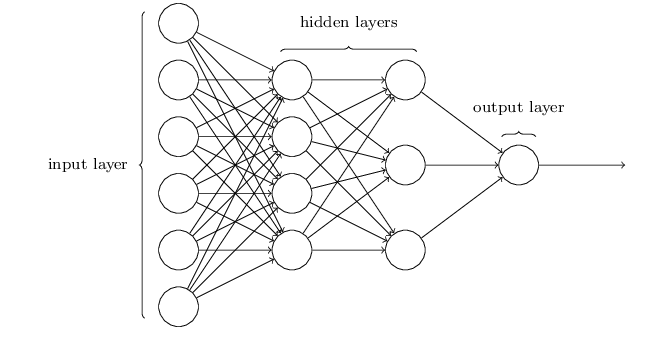
\includegraphics[width=1\linewidth]{project_2/figures/generic_NN.png}
    \caption{Illustration of a generic neural network. \cite[Taken from][Ch.1]{nielsen}.}
    \label{fig:NN}
\end{figure}

A general NN consists of an input layer, $k$ hidden layers and an output layer - all consisting of a varying number of nodes or units, as visualized in Fig. \ref{fig:NN}. The number of nodes in a layer is denoted as the width of the layer, and the number of layers in a network is denoted the depth of the network. 
Hidden layers are not hidden in the sense that they're not a visible part of the model; but rather that when using a trained model one never interacts with anything past the input and output layers, thus the internal nodes appear as hidden. 
Between the nodes we have connections called \textit{weights}. These determine the influence from one particular node to another. 

The weighted model stems from the mathematical function for an artificial neuron given as follows; 

\begin{equation}\label{artifical_neuron}
    y = f\left( \sum_{i=0}^Nwx_i \right) 
\end{equation}

Here $f$ is some \textit{activation function}that takes a weighted sum of $N$ inputs and maps them to an output. Activation functions are further covered in the next subsection, \ref{sec:activation_func}.

How many layers an NN has, how many nodes each layer has and how they're connected make up what's called the \textit{architecture} of the neural network \citep[Ch.1]{nielsen}. These decisions are normally made case-by-case depending on the task at hand, input size, desired output size, etc. Apart from compatible dimensions there are no clear choices for what constitutes a "better" architecture, however more complex tasks are commonly better solved by more "complex" networks; i.e. more layers and more nodes. 


It is sometimes specified wether a network is \textit{fully connected} or not. A fully connected network, or layer, is simply connected in a way that each node receives the output from every single node in the preceding layer. Fig. \ref{fig:NN} is an example of a fully connected NN. However, a fully connected network can always act as a "not-fully connected" network simply by having some of it's weight set to $0$ and thereby nullifying the corresponding connections. 

The simplest model for an artificial neural network is called a \textit{feed forward neural network} (FFNN), where logically enough the flow of information moves only in one direction; forward. Consider for instance a FFNN with one hidden layers. The input-layer receives the input $X$, which is then passed through the first weights $W_0$ to the second layer. Here the weighted sum is passed through an activation function $f_1$ and passed via $W_1$ to the output layer. In the output layer the weighted sum is passed through $f_2$, before finally being output from the model. 
For each node $n$ the process can be formally expressed as:


\begin{equation}
    y = f\left( \sum_{i=0}^N w_{0n}x_i + b\right)
\end{equation}
\citep[p.17]{Ketkar2017}. Here one can clearly see the similarities to Eq. \ref{artifical_neuron}. $b$ represents what is called a \textit{bias term}. Looking back to the structural similarities of a biological NN, the bias allows one to skew "how easy it is to get the neurons to fire". I.e., by altering the bias terms one can shift the the output values in a desired direction - in theory. This is however easier said than done, and directly altering either weights or biases directly are not common procedure. Instead one relies on a good choice of cost function and the training of the NN to produce fitting parameters. 


\subsubsection{Activation functions}\label{sec:activation_func}

The activation functions are the key to how NNs generalize beyond linear methods. As might be inferred, these activation functions should \textbf{not} be linear \citep[p.168]{Goodfellow-et-al-2016}. 
For an NN with one hidden layer and activation functions given as:
\begin{align}
\begin{split}
    f_1(\bold{x})&=\bold{W_0}^T\bold{x} + b_1 \\
    f_2(\bold{x})&=\bold{W_1}^T\bold{x} + b_2 
\end{split}
\end{align}
The entire network could then be expressed: 
\begin{align}\label{linear_nn}
    \begin{split}
        F(\bold{x})&=f_2(f_1(\bold{x})) \\
        &= \bold{W_1}^T(\bold{W_0}^T\bold{x} + b_1) + b_2 \\
        &= \bold{W_1}^T\bold{W_0}^T\bold{x}+\bold{W_1}b_1+b_2 \\
        &=\bold{W}^T\bold{x}+b
    \end{split}
\end{align}
The entire NN itself is just one big chain of all it's weights and activation functions nested. Were the activation functions to be linear, the network itself would be linear (as shown in Eq. \ref{linear_nn}) - undermining the fundamental purpose of an NN. 
Beyond non-linearity there are few hard restrictions on the activation functions, granted some are to be preferred.
The rest of this section will use the convention of $\bold{z}$ representing the vector of "raw output" from the previous layer. Raw output simply refers to the values before they're passed through the activation function. An activation function applied to the entire vector, is simply applied element-wise - i.e. the input and output are congruent and
\begin{equation}
    f(\bold{z})_i = f(z_i)
\end{equation}

One example of a common activation function for classification problems is the Sigmoid function (Eq. \ref{sigmoid}), as used in logistic regression. Tweaking the architecture of an NN, one can deduce that logistic regression is congruent to a FFNN with no hidden layers and the Sigmoid function as the activation function. 

Alternatively the \textit{softmax} function is another common function for classification \citep[Logistic Regression]{morten}. 
This is an extension of the Sigmoid function, and is also what's used in place of the sigmoid function for multinomial linear regression.
The softmax function normalizes a vector of input values so that the resulting outputs sum to $1$. While softmax can be used in internal nodes, it is more commonly used for the output layer. For an input vector of size $K$ the softmax function for each element i is given as: 
\begin{equation}\label{softmax}
f(\mathbf{z})_i = \frac{e^{z_i}}{\sum_{j=1}^K e^{z_j}}
\end{equation}


For internal nodes and some regression tasks the activation function \textit{Rectified Linear Unit} (ReLU) is commonly used \citep[Building a feed forward neural network]{morten}; 
\begin{equation}\label{relu}
    f(\bold{z})_i=\max\{0, z_i\}
\end{equation}
Alternatively ReLU can be expressed as
\begin{equation}
    f(\bold{z})_i = \begin{cases} 
      z_i & \text{if } z_i > 0 \\
      0 & \text{if } z_i \leq 0 
   \end{cases}    
\end{equation}
As opposed to both the sigmoid and the softmax functions, ReLU does not \textit{saturate} for large positive values. The saturation of a function is an issue where the values of the function approaches its maximum or minimum, resulting in vanishing gradients and thereby poor convergence. However, ReLU suffers from an issue called \textit{the dying ReLU}. In essence this refers to nodes stagnating at zero; effectively dying. 

One solution to the problem of the dying ReLU is to use \textit{leaky ReLU} \citep[p. 190]{Goodfellow-et-al-2016}; 
\begin{equation}
    f(\bold{z})_i=\max\{0, z_i\}+\alpha\min\{0,z_i\}
\end{equation}
Here $\alpha$ is typically sat to a small value, like $0.01$. 
Similiar to ReLU, Leaky ReLU can alternatively be expressed as; 
\begin{equation}
    f(\bold{z})_i = \begin{cases} 
      z_i & \text{if } z_i > 0 \\
      \alpha z_i & \text{if } z_i \leq 0 
   \end{cases}
\end{equation}
This variation of ReLU allows for some portion of the negative values to be included, mitigating the risk of dying nodes. 
% Examples: sigmoid, ReLU, leaky ReLU, softmax, identity in last layer?

The output layer of a NN will often have a different activation function than it's predecessors. While the choice of activation functions in the hidden layers have less direct consequences to the type of output, the last activation dictates exactly this. For classification tasks one often has either the sigmoid, the softmax or similar functions for the output layer. Commonly less restrictive functions are used for regression problems, to avoid limiting the possible output scope of the network. Some even choose to use the identity function, or similarly no activation function, for the last layer. 

\subsubsection{Initialization of weights and biases}\label{sec:NN_init}

To start training the NN, and navigating the landscape of the cost function, one needs a starting point \citep[p.297]{Goodfellow-et-al-2016}. For initialization of weights and biases there are a lot of different conventions. How the values are initialized can affect things like the optimization itself, convergence and the generalization of our model. 
One of the most important aspects is to ensure that no nodes are the same; for nodes with the same activation function, same input values and same initial values, most training methods will update these in the same manner. This again will result in a more narrow search field were not all possibilities in the cost landscape can be reached. Although there exists ways to work around this problem it is commonly preferred to avoid this issue as best one can. 
Larger (distinct) initial weights will be more effective against symmetry, but will on the other hand heighten the risk of exploding gradients (section \ref{sec:exploding_gradients}) and saturated nodes (\ref{sec:activation_func}). 


Arguably the most common method across the field, is random initialization. As the wording entails, the weights and biases are then randomly initialized. The values are commonly selected from a Gaussian distribution, with mean zero and standard deviation 1. This method alleviates the chances of symmetrical nodes, while also mitigating the risk of too large weights. Among other methods for initialization many are specialized for specific activation functions, providing benefits like faster convergence and moderation of saturation effects. 

\subsubsection{Choice of cost function for neural networks}
In addition to initialization of weights and biases, the training of the model largely depends on choice of cost function, which again depends on the task at hand. How a cost function looks has in itself no restrictions, but some are more suited than others.
The choice of cost function is arbitrarily what dictates the landscape that is navigated in the optimization of a network. Most popular optimization techniques require a cost function that can be expressed in terms of a loss function, i.e. that can be computed for each data point on its own. 
For networks to be used on regression problems one commonly uses MSE (see section \ref{sec:eval_regression}), and for classification problems cross entropy (section \ref{sec:cross-entropy}) is by far the common choice. 

\subsubsection{Training of the network}
For the actual training of the network, in other words finding the optimal weights and biases, one normally uses gradient descent (see section \ref{sec:gd}). The first step in this process is finding the gradients of the cost function to navigate the parameter landscape. As each layer of a NN can be expressed as a function of its previous layer, one can imagine these expressions to quickly become quite complicated. Furthermore we have to find the partial derivatives for all weights and biases. The most used solution to this intricate problem, is called \textit{backpropagation} \citep[p. 200]{Goodfellow-et-al-2016}. While many libraries provide implementations of automatic gradients, such as PyTorch's Autograd \cite{Ansel_PyTorch_2_Faster_2024} and Tensorflow's GradiantTape \cite{Abadi_TensorFlow_Large-scale_machine_2015}, it is beneficial to understand how manual backpropagation works. Not only is this useful for debugging and ensuring code behaves as expected, but it is essential for understanding the training process. 

The fundamental concept of backpropagation is the use of the chain rule from calculus. Since the network's output is a composition of functions, the chain rule allows us to systematically propagate backwards through the network and compute the derivatives effectively \citep[Ch.2]{nielsen}. 

Denoting the output of layer $(l)$ as $ a^{(l)}$ and the weights and biases for that layer as $W^{(l)}$ and $b^{(l)}$, respectively. For a given layer, the input $z^{(l)}$ to the activation function is:

\begin{equation}
z^{(l)} = W^{(l)} a^{(l-1)} + b^{(l)}
\end{equation}

Here $a^{(l-1)}$ is the output (or activation) from the previous layer. The activation \( a^{(l)} \) is then given by applying the activation function $f$ to $z^{(l)}$:

\begin{equation}
a^{(l)} = f(z^{(l)})
\end{equation}

To calculate how each weight $ W^{(l)}$ and bias $b^{(l)}$ affects the overall cost $L$, we start from the final layer and compute the gradient of the cost with respect to each parameter in the network, working backward through each layer. The gradient of the cost with respect to $W^{(l)}$ is obtained using the chain rule:

\begin{equation}
\frac{\partial L}{\partial W^{(l)}} = \frac{\partial L}{\partial a^{(l)}} \cdot \frac{\partial a^{(l)}}{\partial z^{(l)}} \cdot \frac{\partial z^{(l)}}{\partial W^{(l)}}
\end{equation}

where:
\begin{itemize}[label=--]
    \item $\frac{\partial L}{\partial a^{(l)}}$ is the gradient of the cost with respect to the layer’s activation
    \item $\frac{\partial a^{(l)}}{\partial z^{(l)}}$ is the derivative of the activation function applied at layer $l$
    \item $\frac{\partial z^{(l)}}{\partial W^{(l)}}$ is the derivative of the weighted sum with respect to the weights.
\end{itemize}

By recursively applying this process from the output layer back to the input layer, back-propagation computes all necessary gradients efficiently, enabling gradient descent to adjust each parameter and reduce the cost.

% - Why neural networks
% - 
% \julie{need motivation for NN, one direction FF no loops, input-hidden-output}
% - Backprop
% - The choice of cost function
% - Hidden layers and nodes
% - Activation functions: sigmoid, ReLU, leaky ReLU
% - Should specify why it is important that the activation functions are non-linear
% - Activation function for final layer depends on the application, i.e. regression versus classification
% - Weights and their initialization
% - Initialization of biases  

% \subsection{Resampling methods\mia{copy}}


% When training models, error estimation is crucial both for model selection and model assessment. Without a good metric for the performance of the model it is impossible to gauge how well fit a model actually is.
% Generally, it's desirable to have as much data as possible for the training of a model. When holding off some of the data for testing, this data can then not be used for training. It's therefore of interest to explore methods that allow for a train-test split of the data, while still keeping as much data as possible for training and giving us a better error estimation.

% \subsubsection{Bootstrapping\mia{copy}}
% Bootstrapping is a general term for one such resampling method where one draws with replacement from the original data set, creating a "new" data set for each bootstrap. Every bootstrap sample should have the same size as the original data set, $n$. $B$ such samples are generated, and the training repeated for each of them.
% The $b$-th bootstrap sample produces model $\hat{f}_b$ \citep[p. 249]{hastie}.

% Using bootstrap the estimation of the error can be calculated as follows:
% %the mean of the error across the $B$ bootstrap samples \cite[p. 250]{hastie}:

% \begin{equation}\label{bs_error}
%     BS_{error} = \frac{1}{n}\sum_{i=0}^{n-1} L\left(y_i,\frac{1}{B}\sum_{b=1}^{B} \hat{f}_b(x_i)\right)
% \end{equation}

% \subsubsection{K-fold cross-validation\mia{copy}}
% \textit{K-fold cross-validation} is another method of resampling. 
% The data set is divided into $K$ parts $\mathcal{F}_k$, called folds. 
% The $K$ must be chosen by the developer as they see fit. 
% $K-1$ folds are used as training data, while the remaining fold is used as test data. The model trained when the $k$-th fold is held out, is denoted $f^{k}$. 
% The procedure is repeated $K$ times, holding out a new fold each time. For k-fold cross-validation the estimated error is given as the mean of the $K$ test errors, shown in Eq. \ref{cv_error} \citep[p. 241]{hastie}. Her one takes into consideration that the folds $\mathcal{F}_k$ may be of different sizes.


% \begin{equation}\label{cv_error}
%     CV_{error} = \frac{1}{K} \sum_{k=1}^{K} \frac{1}{|\mathcal{F}_k|} \sum_{i \in \mathcal{F}_k} L\left(y_i, f^{k}({x}_i)\right) 
% \end{equation}

% There are both advantages and disadvantages of this method. On one hand, it achieves the goal of maintaining a train-test split while keeping a sizeable train set. 
% The estimated error (Eq. \ref{cv_error}) will be closer to the true generalization error measure. This is a consequence of the error being averaged over many different models, and thereby to a higher degree taking into account randomness associated with data-selection. 

% On the other hand, cross-validation will be quite computationally costly for a high $K$. Another disadvantage is that there is no clear choice of $K$; here there is a trade-off between bias and variance. A smaller K leads to lower variance, but higher bias. On the other side, a higher K leads to low bias, but high variance. The extreme case of the latter is leave-out-one cross-validation (LOOCV), where every datapoint acts as a fold. It will lead to an unbiased error measure, but the variance will be quite large \citep[p. 242]{hastie}.

\subsection{Scaling}\label{sec:scale}
Scaling data before inputting it to a model is often beneficial, and sometimes a necessity \citep[Linear Regression]{morten}. Some methods, like ordinary least squares, are invariant to scaling and thus it does not affect the performance either way . For methods like ridge regression, which penalizes large coefficients, scaling the data mitigates problems related to parameters of unequal magnitudes being penalized unfairly compared to each other. For neural networks, scaling the data can be beneficial for convergence of the model, and choice of scaler normally depends on the activation functions used in the model \citep[Ch.7]{Goodfellow-et-al-2016}. Additionally models are often sensitive to extreme values / outliers, and scaling our data can help alleviate the effects of this. 

It's considered good practice to not scale the intercept, as it represents a constant term without variability and scaling it will often worsen it's performance, or defeat it's purpose entirely.

A common choice for scaling is to use the \textit{standard scaler}. This method involves subtracting the mean and dividing by the standard deviation, for each feature (i.e. parameter) respectively. Each of the columns will then have mean equal to zero and a standard deviation of one after the scaling. For the $j$-th feature one gets the transformation as 
\begin{equation}\label{standardize}
    \bold{x_j} = \frac{\bold{x_j}-\mu_j}{\sigma_{j}}
\end{equation}
Standard scaling is well suited for methods that assume a underlying normal distribution, such as linear regression. For datasets with large outliers, standard scaling is also beneficial as it makes the data less susceptible to the effects of extreme values.
A variation of the standard scaler is sometimes used, including only subtraction of the mean and omitting the division of standard deviation. This is commonly called \textit{zero centering}. 

Alternatively the \textit{min-max scaler} is another common option. 
\begin{equation}\label{min-max}
    \bold{x_j} = \frac{\bold{x_j}-\min(\bold{x_j})}{\max(\bold{x_j})-\min(\bold{x_j})}
\end{equation}
Max-min scaling is ideal for methods that makes no assumptions about underlying data distributions, like NNs. Shifting the data into the range $[0,1]$ can also be beneficial for convergence of NNs when using activation functions like the sigmoid function. However, it's worth keeping in mind that the min-max scaler is sensitive to outliers. 

% \julie{In order for all parameters to have an equal starting point when training a model, it's often necessary to scale the data \citep[p. 398]{hastie}. Having one parameter with values of order $10^3$, and another parameter with values of order $10^{-3}$, the model could miss the predictive importance of the latter. Whether or not it is necessary to scale the data, depends on the choice of cost function; Given two predictors of different magnitudes where the same relative change has equal impact on the response, the predictors of smaller magnitude would have coefficients of inversely proportional magnitude. If a cost function penalizes bigger coefficients, as some does, the parameter of smaller magnitude would then be penalized more than it should. To alleviate the risk of such problems, it is thus necessary for many methods that all data is scaled before training. 

% A common choice for scaling is to use the \textit{standard scaler}. This method involves subtracting the mean and dividing by the standard deviation, for each feature (i.e. parameter) respectively. Each of the columns will then have mean equal to zero and a standard deviation of one after the scaling. For the i-th datapoint and the j-th feature one gets the transformation as indicated in Eq. \ref{standardize} \citep[Linear Regression]{morten}. Alternatively a variation of the standard scaler is sometimes used, including only subtraction of the mean and omitting the division of standard deviation.

% \begin{equation}\label{standardize}
%     x_{ij} \rightarrow \frac{x_{ij}-\overline{x}_j}{\sigma_{x_j}}
% \end{equation}

% It's considered good practice to not scale the intercept, as it represents a constant term without variability and scaling it will often worsen it's performance, or defeat it's purpose entirely. 
% The intercept may be taken out during training and later be recalculated as Eq. \ref{bet0} shows \citep[Resampling methods]{morten}. 
% Taking out the intercept amounts to removing the column of 1's in the design matrix. 

% \begin{equation}\label{bet0}
%     \beta_0 = \frac{1}{n}\sum_{i=0}^{n-1}y_i - \frac{1}{n}\sum_{i=0}^{n-1}\sum_{j=1}^{p-1}X_{ij}\beta_j
% \end{equation}}

\subsection{Evaluation measures}

\subsubsection{Regression}\label{sec:eval_regression}
\textit{This subsection is reused from our previous work \citep[p. 4]{project1}.}

\begin{equation}\label{mse}
    \text{MSE} = \frac{1}{n}\sum_{i=0}^{n-1}(y_i-\Tilde{y}_i)^2.
\end{equation}

The \emph{mean squared error} (MSE) is a popular error measure for linear regression models, and is defined as in Eq. \ref{mse}, where $n$ denotes the number of data points in the training data, and the prediction for the i-th data point is denoted $\Tilde{y}_i$. Comparing the expression above (Eq. \ref{mse}) to Eq. \ref{cost_ols}, it's clear how the OLS regression method is inherently designed to minimize MSE. 
% Given a loss-function of the squared distance between the prediction and the true value, the errors for cross-validation and bootstrapping (respectively Eq. \ref{cv_error} and Eq. \ref{bs_error}) will trivially be the equivalent of MSE. 

$R^2$ is a measure of how well the model explains the variance present in the data. 
\begin{equation}
    R^2 = 1 - \frac{RSS}{TSS}= 1 - \frac{\sum_{i=0}^{n-1}(y_i-\Tilde{y}_i)^2}{\sum_{i=0}^{n-1}(y_i-\overline{y}_i)^2},
\end{equation}

$R^2 \in (-\infty,1]$. If $R^2 = 1$ the model perfectly explains all variance, whereas a value of 0 would mean does not explain any of the variance. 
A prediction $\tilde \y = \bar \y$, would result in $R^2 = 0$.
If $R^2<0$, the model is worse than a straight line.
The numerator is the sum of the squared residuals, also called RSS. The denominator is the total sum of squares, in short TSS \cite[p. 29]{martin}.

\subsubsection{Classification}
While the mean squared errors and $R^2$ measures could give us a rough grasp about the quality of a classification model, there are several other methods better suited to measure the model's performance.
One such measure is \textit{accuracy}.
\begin{equation}\label{eq:acc}
    \text{accuracy} = \frac{\text{correct predictions}}{\text{total predictions}}
\end{equation}
Accuracy is simply defined as correct predictions divided by total predictions (see Eq. \ref{eq:acc}), and is a good measure on how often the model is correct.
There is however an important weakness with accuracy, especially for certain types of data.
This stems from the fact that the two types of errors in a binary classification model, \textit{false positives} and \textit{false negatives}, are in many cases not equally bad.
Furthermore, many data sets are very skewed, with one outcome having many more data points than the other.
A prime example of this is models based on medical data sets, trying to predict whether a patient has some disease, such as the Wisconsin breast cancer data set \cite{breast_cancer_wisconsin}.
Clearly, in most of these cases, it is worse if the models wrongly predict that a sick patient is healthy, than the other way around.

\begin{table}[h]
    \centering
    \begin{tabular}{|m{8em}|m{8.5em}|m{8.5em}|}
    \hline
        \diagbox[width=8em]{\textbf{Truth}}{\textbf{Predicted}} & \textbf{Disease} & \textbf{No disease} \\
    \hline
        \textbf{Disease} & true positive (TP) & false negative (FN) \\
    \hline
        \textbf{No disease} & false positive (FP) & true negative (TN) \\
    \hline
    \end{tabular}
    \caption{Confusion matrix for medical data}
    \label{tab:conf_mat}
\end{table}

An example is the Norwegian mammography program, where only 3\% of the initially tested will receive follow up tests or treatment \cite{kreft_reg}.
In this case, a model predicting everyone to be healthy would obviously be very bad, however it would get an accuracy score of 0.97, which is considered very good.
It is also much worse to send a person with the disease home, than to send a healthy person to a follow-up consultation.
Hence we need a better solution to measure the quality of the model.

A naive solution that solves the problem of skewed data sets, is removing data points from the majority set, in order to make the data set less skewed.
This often a bad solution for two reasons.
It reduces the original dataset by a lot of data points (in the Norwegian mammography program example a completely equally distributed data set would contain at most 6\% of the data points), which is of course much worse for training the model.
Secondly, it does not consider the fact that the two different error types are not equally bad.

\begin{align}
    \label{eq:precision} \text{precision} &= \frac{\text{TP}}{\text{TP}+\text{FP}} \\
    \label{eq:recall} \text{recall} &= \frac{\text{TP}}{\text{TP}+\text{FN}}
\end{align}

For these kind of models, measures such as \textit{precision} and \textit{recall} are popular.
They both focus on the true positives, and ignore true negatives (see table \ref{tab:conf_mat}).
Precision (Eq. \ref{eq:precision}) is the fraction of predicted positives where the true values are positive, while recall (Eq. \ref{eq:recall}) is the fraction of positive cases that are predicted positive by the model \citep[p. 418]{Goodfellow-et-al-2016}.
The equations uses the definitions of true positives (TP), false positives (FP) and false negatives (FN) as shown in table \ref{tab:conf_mat}.
Clearly, recall is an important measure for medical cases, as you do not want to send home sick patients.
That being said, a model must also have a certain level of precision in order to be useful. Predicting every instance to be true, would yield a high recall value - but trivially it would not be a very helpful model.
\begin{equation}\label{eq:fscore}
    F = \frac{2\cdot \text{precision} \cdot \text{recall}}{\text{precision} + \text{recall}}
    = \frac{2 \text{TP}}{2 \text{TP}+\text{FP}+\text{FN}}
\end{equation}

A compromise between precision and recall is the \textit{F-score} (Eq. \ref{eq:fscore}).
An F-score close to 1 suggests that the model is good, while an F-score close to 0 is a sign of a bad model.
Even though the F-score is good at evaluating the quality of a binary classification model, it provides little about what is wrong with the model, giving you no insight to if the error stems from the precision or the recall, or both.
Hence, one will have to also calculate the precision and recall separately to figure out why a model has a low F-score.

% \subsection{\mia{MIA THINGS}}
